\chapter{Indoor applications using autonomous drones}
\label{cap3}

In this Chapter we show all the problems we had to face in the development of our programming framework. 
We first show a concrete application we wanted to develop, and then the problems deriving from its development.
No one of the existing drone programming approaches, shown in Chapter \ref{cap2}, is fully suitable for our problem.
We chose a Team-level programming approach, described in Section \ref{teamlevel}, but we had to perform some modifications on it, as we explain in Section \ref{teamlevelproblems}.
There are also some technological limitations, such as the lack of a stable indoor localization system and the short duration of nano-drones battery, which we explain in Section \ref{challenges}.

\section{Motivating scenario\label{motivating}}

In order to concretely show all the limitations and problems encountered in the development of our system, we start this Chapter describing a concrete scenario.
We want to develop an application to assist elders to take their medicines, for example in a hospital context.
A team of nano-drones could help the nurses to deliver the daily medicines to the patients at the right time of the day.
A representation of the behavior of the application, which we named Drugs Distribution(DD), is shown in figure \ref{fig:motivating}:


\begin{itemize}
\itemsep2pt
\item{
the nurses prepare the little boxes with each patient’s daily medicine
}
\item{
each drone, at the right time of the day, brings the box to its assigned patient
}
\item{
after carrying out their action, the drones return to the start location
}

\end{itemize}


\begin{figure}[H]
  \centering
  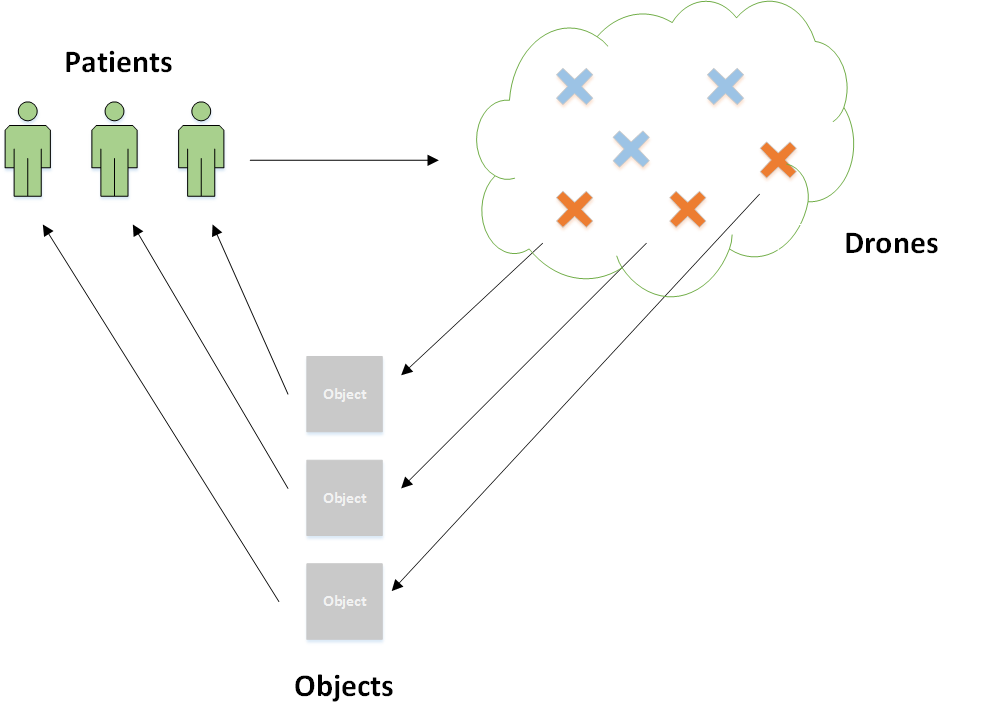
\includegraphics[width=\linewidth]{pictures/DD.png}
  \caption{The basic functioning of the Drugs distribution application}
  \label{fig:motivating}
\end{figure}

The development of this application made us to face some problems, both in the implementation of the system and in the technological lacks, which we describe in the next two Sections.


\section{Drone programming}\label{teamlevelproblems}

Since the approaches for programming drones we described in chapter \ref{cap2} are designed in a way that is impossible to describe an application through the concepts of Mission and Trip, we give our contribution to the state of the art creating a new framework based on these entities.
A \textit{Mission} is nothing but a list of sensing tasks to be performed sequentially in the environment.
Each one of these sensing tasks is a \textit{Trip}, that is a movement from a point A to a point B to perform an Action.

Neither the Drone-level nor the swarm-level approaches, described in Sections \ref{droneLevel} and \ref{swarmLevel} respectively, are suitable for our goal. 
The former because we do not want the user to deal with the coding of each drone separately with an external API.
The latter because we want to avoid the complexity to create a communication network protocol between drones and because it would be difficult to maintain the status of the missions and trips entities among the swarm. Moreover we also need to address  time and space constraints, which cannot be expressed with this approach.
\\

The most suitable approach for our framework is the Team-level model, described in Section \ref{teamlevel}, but we need to apply some modifications to it, in order to make it suitable for our work.
Using a Team level approach entails some problems:
the user can neither address individual drones nor express actions that involve direct interactions between drones, such as those required to pass an object between them.
This is the main limitation of the approach, but it does not directly affect the development of our DD application, described in Section \ref{motivating}.
So we have to modify the Team-level approach in order to make each drone deliver the box of medicine to its assigned patient, independently from the other drones. 
So we need the concept of \textit{Trip}.
A \textit{Trip} is nothing but a movement from a point A to a point B in the environment to perform an action.
In this way, we can tell each drone to go to the precise location of its assigned patient, making the Trip of each Drone independent from the others.
The concept of \textit{Trip} is a fundamental feature of our model, and it is fully described in Section \ref{programmingModel}.
\\

Another very important feature of our system is the transparent dispatching of drones:
the central brain takes care of assigning the drones to the sensing tasks to be performed, managing also the drones failures, without involving the programmer.
\\

Another problem of the Team-level approach is that, having a single brain which manages all the application logic and the dispatching of drones, the system get a single point of failure, so, if the central brain breaks then the whole system crashes.
This problem can be fixed or at least weakened by applying some dependable systems methods, improving reliability of the central brain, reducing its rate of failure etc.
\\

Even though team-level approach has his own limitations, other approaches we discussed in Chapter \ref{cap2} are less suitable.
Indeed, the Drone-oriented approach, described in Section \ref{droneLevel}, has the problem that the programmer has to manage individually the drone's movements and the interactions with other drones: he must code a list of instructions and commands that the drone will perform sequentially. This can only be achieved with the exploiting of specific API of each drones.
In the case of multiple drones,the programmer should deal with difficult programming tasks, like concurrency and parallelism, and it should also manage the drone batteries discharge and their crashes/failures.
Adding one or more drones to the system could complicate a lot the programming task. The programmer should also deal with timing constraints and he should balance the load between drones in a dynamic way.
Is clear that the drone-level approach is most suitable for applications involving only a few drones.
\\

On the other hand, the Swarm-level approach, described in Section \ref{swarmLevel}, is more suitable for applications where there’s need of a lot of drones performing the same actions.
Indeed the programmer can give a set of basic rules that each drone should follow. It is important to underline that, in swarm-level approach, there is no possibility to have a shared state between drones; each one execute the actions specified by the programmer on his own local state. This means that this approach is very easy to scale up adding new drones, but it’s not suitable for applications that require the drones to explicitly coordinate.
\\

Regarding the dataflow programming, we need a new framework that allows the user to design the behavior of the central brain taking care of the missions execution, from the beginning to the end. 
This modeling tool helps the developer to add the features needed by the application simply drawing the proper nodes in the dataflow graph. 
The BPMN and Node-RED dataflow models, described in Sections \ref{BPMN} and \ref{NodeRed} respectively, are too general for our system, since they allow to model almost every kind of project.
They offer a great number of components, but we only need basic components for our editor, like rectangles and arrows.
So we decided to develop our own dataflow model, offering only the functionality and components needed for our programming framework.
This part of the project is fully described in Section \ref{plutoGraphicalEditor}.

\section {Implementation challenges}\label{challenges}

The DD application, shown in Section \ref{motivating}, makes drone bring medicines to the elders in an hospital, so in an indoor context.
One big problem is that there is not a stable localization method for the indoor environment.
Besides of localization problem, indoor context also leads to the limits of the size of the drone.
As a result, programmers constantly confront with a limited battery resource and a small weigh the drone can carry out. These problems, as well as their possible solutions, are described in the following Section.

\subsection{Indoor localization}\label{indoor}

The main issue that all developers are facing, working on an indoor application for drones, is that they are not able to use the Global Positioning System (GPS); it cannot be used because of walls,roofs or ceilings.
For this reason Indoor Positioning System(IPS) is widely applied for indoor localization. In this Section we will give an overview of existing IPS methods.  
\\

An indoor positioning system is a solution to locate objects or people inside a building using radio waves, magnetic fields, acoustic signals, or other information collected from the sensors of mobile devices.
The IPS methods rely on alternative technologies, such as \textit{magnetic positioning} and \textit{dead reckoning}, to actively locate mobile devices and provide ambient location for devices to get sensed.

Today many IPS methods have been developed and they can be divided in two main categories: \textit{Non-radio technologies} and \textit{Wireless technologies}.
\\

Non-radio technologies have been developed for localization without using the existing wireless infrastructures, and they can provide very high accuracy.
Nevertheless, they also require expensive installations and costly equipment.
\\

For example, \textit{Magnetic positioning}\cite{magnetic} is based on the iron inside buildings that create local variations in the Earth’s magnetic field.
Modern smartphones can use their magnetometers to sense these variations in order to map indoor locations.
\\

With \textit{Inertial measurements}\cite{IMU} pedestrians can carry an inertial measurement unit(IMU) by measuring steps indirectly or in a foot mounted approach, referring to maps or additional sensors to constrain the sensor drift encountered with inertial navigation.
\\

Existing wireless infrastructures can be used for indoor localization; almost every wireless technology is suitable, although they are not as precise as non-radio technologies.
Localization accuracy can be improved at the expense of new wireless infrastructure equipment and installation.
WiFi signal strength measurements are extremely noisy, so there is need to find a way to make more accurate systems by using statistics to filter out the inaccurate input data. WiFi Positioning Systems are sometimes used outdoors as a supplement to GPS on mobile devices, where only few reflection phenomena could happen.
\\

\textit{WPS}\cite{WPS} is based on measuring the intensity of the received signal(RSS) together with the technique of \textit{fingerprinting}.
In computer science, a fingerprinting algorithm is a procedure that maps an arbitrarily large data item to a much shorter bit string, its fingerprint, that uniquely identifies the original data for all practical purposes just as human fingerprints uniquely identify people for practical purposes.
The accuracy of WPS improves with the increase of the number of positions entered in the database.
WPS is subjected to fluctuations in the signal, that can increase errors and inaccuracies in the path of the user.
\\

\textit{Bluetooth}\cite{bluetooth} cannot provide a precise location, since it's based on the concept of \textit{proximity}, indeed it is considered an \textit{indoor proximity solution}.
However, by linking micro-mapping and indoor mapping to Bluetooth and through the usage of \textit{iBeacons}, real existing solutions have been developed for providing large scale indoor mapping.
\\

It is important to underline that we made the choice to decouple the system working logic from the \textit{Navigation System}. The navigation system is the module of our central brain that makes use of indoor localization API, providing to the central brain a way to control the drones with accurate coordinates. In this way all previously described technologies are suitable with our system, on condition that the developer provides the proper API.
\\

\subsection{Drones and Objects size limitation}

Indoor contexts imply small areas which are usually full of people and obstacles hence, drones have to be small, in order to avoid crashes with both human and environmental obstacles.

Size limitations result in many problems; the first is battery duration, which can reach a maximum of 8 minutes, having a recharge time of about 20/30 minutes.
It limits the programmer in developing applications which require the drones to perform their actions in this limited amount of time.

Another problem arising from size limitations is that the smaller the drone is the less stable he is.
Almost every kind of micro-drone has serious stability issues, and a lot of research efforts goes in this direction. This problem is lowered by the developing of programming libraries that could improve stability of the drones at real-time, adjusting a set of parameters while the drone is flying.

Micro-drones are obviously more fragile than the big ones, so a crash with humans or obstacles can definitely destroy the drone or make it seriously damaged. This is the price to be paid for having little drones that can operate in small indoor contexts.

Finally, the use of small drones means that only small objects can be taken, so the applications developed with Pluto framework must take this into account.
For example, a pair of keys can be brought to a person, not a book nor a pair of shoes.